\section{Resultados}\label{sec:sensres}

\begin{table}[htbp]
\centering
\caption{Resumen de la sensibilidad. Cambio de costo de la matheurística respecto de los datos originales de la misma semana, ahorro frente al caso base en el escenario y cambio medio en las solicitudes externalizadas por la matheurística. El detalle por semana está en el Apéndice~\ref{ap:sensibilidad}.}\label{tab:sensibilidad}
\footnotesize
\begin{tabular}{lcccc}
\toprule
Escenario & Semanas & Cambio de costo & Ahorro frente al caso base & Cambio en externalizadas \\
\midrule
\tabinput{tablas/sens_resumen.tex}
\bottomrule
\end{tabular}
\end{table}

\parrafo{La ventaja se mantiene.} La Tabla~\ref{tab:sensibilidad} resume las corridas, todas validadas sin errores. La matheurística es más barata que el caso base en todos los escenarios y semanas, con ahorros entre 5,0 y 14,0\,\%. Ningún supuesto evaluado hace desaparecer el beneficio de coordinar. Los ahorros más bajos aparecen cuando hay mucha externalización (sin división, con más demanda o con externalización barata): esa parte del costo la pagan casi por igual ambos métodos y queda menos ruteo que optimizar.

\begin{figure}[htbp]
\centering
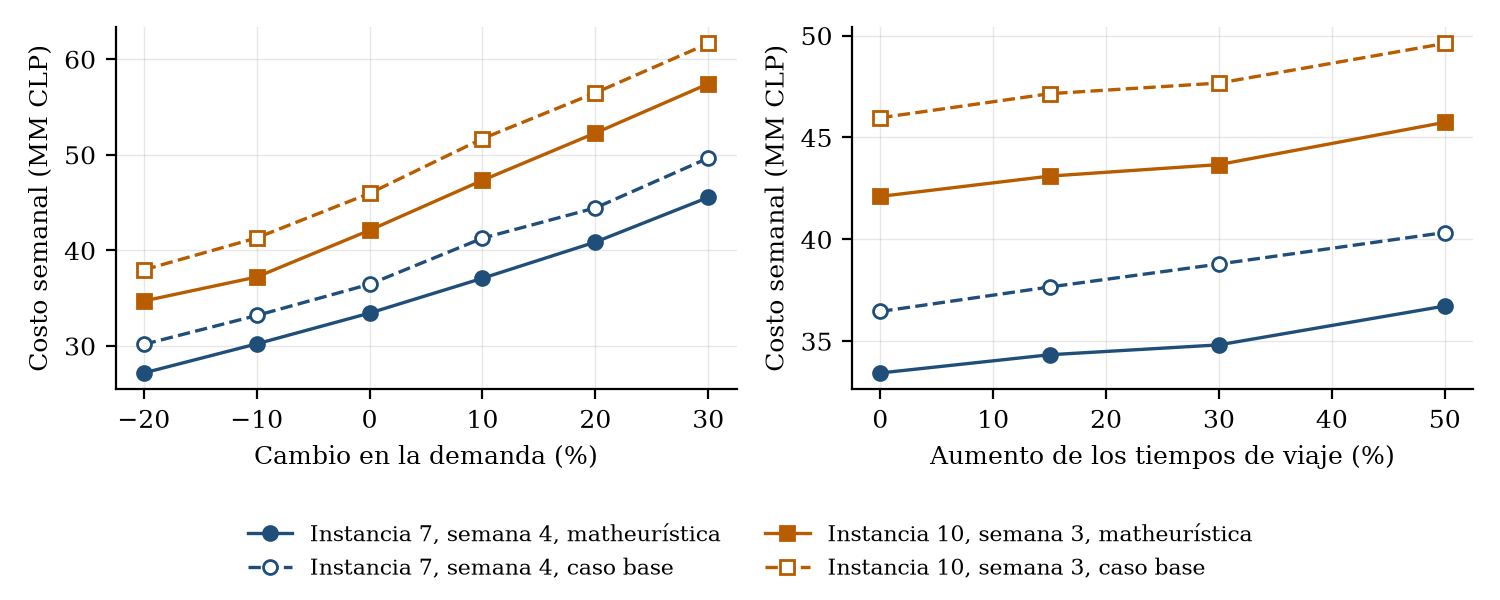
\includegraphics[width=\textwidth]{figures/fig_demanda_congestion.png}
\caption{Costo semanal según el cambio en la demanda (izquierda) y en los tiempos de viaje (derecha), en las semanas mediana y de mayor demanda.}\label{fig:demcong}
\end{figure}

\parrafo{Demanda: el costo crece cada vez más rápido.} La Figura~\ref{fig:demcong} muestra que el costo responde a la demanda de forma convexa. En la semana mediana, la demanda $-20$, $-10$, $+10$, $+20$ y $+30$\,\% cambia el costo de la matheurística en $-18{,}7$, $-9{,}6$, $+10{,}9$, $+22{,}2$ y $+36{,}2$\,\%. Bajar la demanda ahorra menos que proporcionalmente, porque los costos fijos de bases y parte de la flota se mantienen; subirla cuesta más que proporcionalmente, porque la flota casi no puede crecer donde hace falta. La respuesta depende de la holgura de la semana: con $+20$\,\%, el costo sube un 16,7\,\% en la de menor demanda, donde sobran vehículos, y un 27,9\,\% en la instancia 8, donde los 18 furgones ya estaban ocupados y las externalizaciones pasan de 21 a 42. Por la misma razón el ahorro frente al caso base baja con la demanda, hasta 6,8\,\% con $+30$\,\% en la semana más exigente.

\parrafo{Flota.} Retirar un cuarto de los vehículos sube el costo entre 2,5 y 5,8\,\% (hasta \$2,6 millones por semana). Con solo 14 furgones, la matheurística contrata más vans y externaliza en promedio 12 solicitudes más, aunque bastante menos que el caso base en la misma situación (17 contra 28 en la semana mediana). En la semana de menor demanda el efecto es pequeño (2,5\,\%), porque la flota completa no se usaba. Este escenario y el de demanda apuntan al mismo recurso: el furgón frío.

\parrafo{Tiempos de viaje.} Una congestión de 15, 30 y 50\,\% sube el costo entre 2,4 y 2,7\,\%, entre 3,7 y 6,5\,\% y entre 8,6 y 11,4\,\%, respectivamente. Hasta un 30\,\% la red absorbe el cambio agregando entre dos y cuatro vehículos; con 50\,\% las externalizaciones crecen, sobre todo en la instancia 8 (de 21 a 31). Como los tiempos usados suponen flujo libre, los costos reportados en el Capítulo~\ref{cap:trabajo} deben leerse como un piso: si los viajes fueran entre 15 y 30\,\% más lentos, el costo sería entre 2 y 7\,\% mayor, pero la ventaja de la matheurística se mantiene.

\parrafo{Ventanas de atención.} Alargar en 30 minutos el cierre de cada ventana baja el costo un 3,5\,\% en la semana mediana y un 4,6\,\% en la de mayor demanda, con la misma flota; el ahorro viene casi entero de las externalizaciones, que pasan de 8 a 1 y de 20 a 6. Acortarlas en 15 minutos sube el costo un 2,7 y un 2,6\,\%, y las externalizaciones suben a 12 y 23. La respuesta es asimétrica: media hora más de holgura vale más que lo que cuestan 15 minutos menos. Las ventanas cortas son justamente lo que vuelve difíciles a los insumos grandes (Sección~\ref{sec:resultados}), por lo que negociar ventanas más amplias con los centros que más externalizan es una alternativa barata a contratar más furgones.

\parrafo{Jornada y puntualidad.} Partir la jornada a las 07:00 baja el costo entre 0,1 y 4,1\,\%. El efecto es mayor en la semana de menor demanda, donde permite atender antes de las 08:00 los retiros tempranos con tres vehículos menos, y casi nulo en la semana mediana. Prohibir todo atraso no encarece la operación: el costo cambia entre $-1{,}5$ y $+0{,}5$\,\% y las entregas atrasadas bajan a cero. Esas diferencias son del orden de la variación que produce cualquier cambio en los datos sobre la búsqueda heurística, por lo que se interpretan como costo nulo. La matheurística atrasaba entregas porque la penalización por minuto era menor que el costo del desvío, no porque no pudiera evitarlo, de modo que la organización puede exigir puntualidad total sin pagar más.

\parrafo{Costo de externalizar.} Si externalizar cuesta la mitad, la matheurística externaliza en promedio 40 solicitudes más por semana y baja su costo entre 5,6 y 10,5\,\%. Si cuesta el doble, externaliza casi lo mismo (2 solicitudes menos en promedio) y el costo sube entre 3,9 y 11,0\,\%: esas solicitudes no se pueden atender con la flota disponible a un precio razonable, lo que confirma el diagnóstico de la Sección~\ref{sec:resultados}. La ambigüedad del dato cambia el nivel de costo, pero no la estructura de la solución ni la ventaja del método.

\parrafo{Bases.} Con el costo de las bases duplicado, la matheurística sigue usando las nueve en las cuatro semanas y su costo sube entre 3,1 y 4,4\,\%, casi exactamente el costo fijo agregado: cada base cuesta entre \$130.000 y \$185.000 por semana, menos que los kilómetros que ahorra tener los vehículos cerca de la demanda. La capacidad de las bases tampoco limita: con $+50$ o $-25$\,\% el costo cambia entre $-0{,}4$ y $+0{,}6$\,\%, se siguen usando las nueve bases y el mismo número de vehículos. Aunque Macul y Talagante quedan llenas en 23 de las 40 semanas, los vehículos que no caben se ubican en bases vecinas casi sin costo adicional.

\parrafo{Coordinación (objetivo O5).} Ofrecer planes de transferencia para todas las solicitudes transferibles cambia el costo entre 0 y 0,8\,\% y no aumenta el uso de hubs. Las transferencias casi no se usan porque, con estos datos, el desvío hacia un hub y la espera del intercambio rara vez compensan frente a una ruta directa, y no por la forma de generar los planes. La división, en cambio, es el supuesto que más vale de toda la sensibilidad. Sin ella el costo sube un 35\,\% en la semana mediana y un 32\,\% en la de mayor demanda, y las externalizaciones pasan de 8 a 125 y de 20 a 158. Casi todas (120 y 150) son solicitudes cuya cantidad supera la capacidad de cualquier vehículo compatible, que sin división solo se pueden externalizar. El ahorro frente al caso base baja a 5,0 y 6,2\,\%, porque esa externalización la pagan ambos métodos. De las dos formas de coordinación, la división es la que sostiene la operación con estos datos; los hubs aportan poco.

\parrafo{Utilización del caso base.} Con una utilización de 60, 70, 80, 90 y 100\,\% para dimensionar su flota inicial, el caso base cuesta en promedio 40,15, 39,38, 39,03, 38,85 y 38,85 millones por semana en las 40 semanas BIG: desde 80\,\% el ajuste de flota compensa la diferencia. Contra el mejor de ellos, el ahorro de la matheurística sigue siendo de 9,5\,\%, de modo que la comparación no depende de ese parámetro.

\parrafo{Implicancias.} Las conclusiones del Capítulo~\ref{cap:trabajo} son robustas: la ventaja de coordinar se mantiene en todos los escenarios, y la estructura de la solución (nueve bases, furgones como recurso escaso, hubs casi sin uso) cambia poco. La excepción es la división de solicitudes, sin la cual la operación se encarece en un tercio. Lo que más mueve el costo es lo que la organización controla menos, la demanda y la congestión, y en ambos casos la red se vuelve más cara justo cuando se agotan los furgones. Entre lo que sí controla, exigir puntualidad total y adelantar la jornada tienen costo nulo o negativo, mientras que el precio de externalizar define cuánto conviene sostener con flota propia.
